\documentclass[plainarticle,zihtitle,german,final,hyperref,utf8]{zihpub}
\usepackage{setspace}
\usepackage{listings}
\author{Bengt Lennicke}
\title{Komplexpraktikum "Paralleles Rechnen" \newline A - Stringmanipulationen mit Intrinsics}




\begin{document}

\section{Aufgabenstellung}

Implementieren Sie eine sequentielle und eine SIMD-parallele (mittels Intrinsics für einen Prozessor, der AVX2, AVX und FMA unterstützt) Variante für folgende String-Funktionen:
\begin{verbatim}
/* turns string "string" (with length len_string) to uppercase */
/* returns 1 if there has been an error, 0 if there has been no error */
int toUppercase(char* string, int len_string)

/* turns string "string" (with length len_string) to lowercase */
/* returns 1 if there has been an error, 0 if there has been no error */
int toLowercase(char* string, int len_string)

/* counts the appearences of character "c" in string "string" */
/* (with length len_string) */
/* returns -1 if there has been an error, and the number of appearences*/
/* if there has been no error */
int countChar(char* string, int len_string, char c)
\end{verbatim}
\begin{itemize}
	\item Beschreiben Sie für diese Funktionen die asymptotische Zeitkomplexität.
	\item Messen und Vergleichen Sie die Ausführungszeiten für sequentielle und SIMD-parallele Ausführung für Strings der Länge 10.000, 100.000, 1.000.000 und 100.000.000 .
	\item Nutzen Sie dafür die "romeo" Partition von taurus.
	\item Führen Sie jeweils 20 Messungen durch und analysieren Sie die Ergbenisse mit geeigneten statistischen Mitteln.
	
\end{itemize}

\section{Umsetzung}
\subsection{string\_manipulation.c}
Das Programm ist aufgeteilt in Dateien für den sequentiellen und parallelen Ansatz und einer 'main'-Datei, welche die Laufzeitmessungen für beide Umsetzungen durchführt. Die 'main'-Datei ist 'string\_manipulation.c'. Der Anfang der 'main'-Funktion darin ist im folgenden zu sehen.

\label{code:main} % TODO is there a better way to do this?
\begin{lstlisting}[language=c, numbers=left]
	int main()
	{
		int len_string; 	
		FILE *file;
		
		init_register();
		
		// 10000
		file = fopen("../evaluation/data/string_times_10000.csv", "w");
		if (measurement(file, 100, 10000))
		{
			return 1;
		}
		fclose(file);
		
		// 100.000
		...
	}
\end{lstlisting}

Zunächst werden einige Register initialisiert (\ref{code:main} line 6), welche für die parallelen Berechnungen notwendig sind. Näheres dazu im Kapitel \ref{subsec:par}. Anschließend wird für die jeweiligen Stringlängen (10.000, 100.000,...) eine csv-Datei geöffnet (line 9) und die "measurement"-Funktion aufgerufen.

\begin{lstlisting}[language=c, numbers=left]
	int measurement(FILE *file, int iterations, int len_string)
	{
		char *string;
		int i;
		string = rand_string_alloc(len_string);
		fprintf(file,
		"count_par,count_seq,upper_par,upper_seq,lower_par,lower_seq\n");
		for(i = 0; i < iterations; i++)
		{
			
			if (measure(file, string, len_string))
			{
				return 1;
			}
		}
		free(string);
		return 0;
	}
	
\end{lstlisting}

In der 'measurement'-Funktion wird ein zufälliger String mit gegebener Länge wird erstellt.
Das Ergebnis der Messung wird in Form einer csv-Datei festgehalten. Daher wird die Header-Zeile mit den Spaltennamen in die übergebene Datei geschrieben (line 6-7). Die Spaltenamen sind in der Reihenfolge der Messungen in der 'measure' Funktion.
Anschließend wird 'iterations'-mal mit dem gebildeten String die 'measure'-Funktion aufgerufen.

Die 'measure'-Funktion führt für den gegebenen String die sequentiellen und parallelen Funktionen für 'toUppercase', 'toLowercase' und 'countChar' aus und schreibt die gemessenen Laufzeiten in die gegebene Datei im csv Format.
\begin{lstlisting}[language=c, numbers=left]
	int measure(FILE *file, char *string, int len_string)
	{
		int par_count, seq_count;
		struct timespec start, end;
		
		// string gets changed so we work with duplicates to be able to reset
		char *seq_string, *par_string;
		seq_string = malloc(len_string * sizeof(char));
		par_string = malloc(len_string * sizeof(char));
		strncpy(seq_string, string, len_string);
		strncpy(par_string, string, len_string);
\end{lstlisting}

Da die jeweiligen Stringverarbeitungsfunktionen mit Pointern auf den String arbeiten und den gegebenen String inplace verarbeitet wird, wird in line 8-11 der String in neu-allokiertem Speicher kopiert.
Es wird für se­quen­ti­ell und parallel jeweils ein String vorbereitet, damit die Ergebnisse der Funktionen vergleicht werden können, um die Korrektheit der Ansatze zu versichern.

\begin{lstlisting}[language=c, numbers=left]		
		// start with count as no reset necessary after
		// count
		clock_gettime(CLOCK_MONOTONIC, &start);	
		par_count = countCharPar(par_string, len_string, 'c');
		clock_gettime(CLOCK_MONOTONIC, &end);
		fprintf(file, "%d,", time_diff_in_ns(start, end));	
		
		clock_gettime(CLOCK_MONOTONIC, &start);	
		seq_count = countCharSeq(seq_string, len_string, 'c');
		clock_gettime(CLOCK_MONOTONIC, &end);
		fprintf(file, "%d,", time_diff_in_ns(start, end));	
		if (par_count != seq_count)
		{
			fprintf(stderr, "Counting does not match up.\n");
			return 1;
		}
\end{lstlisting}

Die erste Messung ist für die 'countChar' Funktion. Diese Funktion verändert den übergebenen String nicht, daher können 'seq\_string' und 'par\_string' für die Messung danach nochmal verwendet werden. Die Zähl-Messung zu Beginn spart daher einmal das erneuern der Strings.

Für die Messung der Zeit wird mit der 'clock\_gettime'-Funktion aus der 'time.h' Bibliothek vor und nach dem Funktionsaufruf verwendet. Ich habe die clockid 'CLOCK\_MONOTONIC' gewählt, weil ich diese im Zusammenhang mit 'Laufzeitmessungen in C' am meisten gefunden habe und es funktioniert hat. Inhaltlich würden hier auch andere möglich seien.

Der Unterschied zwischen den beiden Zeitstempeln in Nanosekunden wird dann in die übergebene Datei geschrieben, jeweils mit einem Komma dazu für das csv-Format.

Es wird zunächst die Laufzeit der 'countCharPar'-Funktion in line 3-6 gemessen und geschrieben; analog in line 8-11 für die Funktion 'countCharSeq'.

Anschließend werden die Ergebnisse verglichen und die Funktion bricht ab, wenn beide Ansätze nicht zum gleichen Ergebnis gekommen sind.
		
\begin{lstlisting}[language=c, numbers=left]		
		// uppercase
		clock_gettime(CLOCK_MONOTONIC, &start);	
		toUppercasePar(par_string, len_string);
		clock_gettime(CLOCK_MONOTONIC, &end);
		fprintf(file, "%d,", time_diff_in_ns(start, end));	
		
		clock_gettime(CLOCK_MONOTONIC, &start);	
		toUppercaseSeq(seq_string, len_string);
		clock_gettime(CLOCK_MONOTONIC, &end);
		fprintf(file, "%d,", time_diff_in_ns(start, end));	
		if (strcmp(par_string, seq_string))
		{
			fprintf(stderr, "toUppercase does not match up.\n");
			return 1;
		}
		
		// reset
		strncpy(seq_string, string, len_string);
		strncpy(par_string, string, len_string);
\end{lstlisting}		

Die Messung für die 'toUppercase' Funktionen verläuft analog zum Fall darüber. Allerdings werden hier die übergebenen Strings verändert. Damit die 'toLowercase' Funktionen nicht mit reinen Großbuchstaben-Strings arbeiten sondern ebenfalls mit dem in der 'measurement'-Funktion Bestimmten, werden 'seq\_string' und 'par\_string' zum Schluss  resettet.

\begin{lstlisting}[language=c, numbers=left]		
		// lowercase
		clock_gettime(CLOCK_MONOTONIC, &start);	
		toLowercasePar(par_string, len_string);
		clock_gettime(CLOCK_MONOTONIC, &end);
		fprintf(file, "%d,", time_diff_in_ns(start, end));	
		
		clock_gettime(CLOCK_MONOTONIC, &start);	
		toLowercaseSeq(seq_string, len_string);
		clock_gettime(CLOCK_MONOTONIC, &end);
		fprintf(file, "%d\n", time_diff_in_ns(start, end));	
		if (strcmp(par_string, seq_string))
		{
			fprintf(stderr, "toLowercase does not match up.\n");
			return 1;
		}
		
		free(par_string);
		free(seq_string);
		return 0;
	}
	
\end{lstlisting}

Anschließend findet noch die Messung für die 'toLowercase' Funktionen statt.
Hier wird in line 10 anstelle des Kommas ein Zeilenumbruch in die csv-Datei geschrieben, da die Ergebnisse der nächsten Messung in die nächste Zeile gehören.


\subsection{string\_manipulation\_seq.c}
Die Funktionen 'countCharSeq', 'toUppercaseSeq' und 'toLowercaseSeq' sind in 'string\_manipulation\_seq.c' definiert.

\begin{lstlisting}[language=c, numbers=left]
	int toUppercaseSeq(char *string, int len_string)
	{
		while(*string)
		{
			*string = toupper(*string);
			*string++;
		}
		return 0;
	}
	
\end{lstlisting}

Im sequentiellen Ansatz wird der String sowie die Stringlänge übergeben. Die Übergabe der Stringlänge war in der Aufgabenstellung gefordert, wird aber nicht benötigt.

In der Funktion gibt es einen while-loop, welcher durchläuft solange der Pointer '*string' nicht '\0' ist. Dieses Zeichen markiert das Ende von Strings, sodass der Loop arbeitet bis der Pointer auf das Ende des Strings zeigt.

Im Loop wird das Zeichen worauf der Pointer aktuell zeigt ersetzt, durch das Ergebnis der 'toupper'-Funktion aus der 'ctype.h' Bibliothek (line5). Diese Funktion nimmt ein Zeichen und wenn es ein lowercase Charakter ist, dann wird der passende uppercase Charakter zurückgegeben. Anschließend wird der Pointer auf das nächste Zeichen im String bewegt und der Loop beginnt erneut (line 6).

Die Funktion 'toLowercaseSeq' funktioniert exakt analog und unterscheidet sich nur in line 5; dort wird 'tolower' anstelle von 'toupper' verwendet.

\begin{lstlisting}[language=c, numbers=left]
	int countCharSeq(char *string, int len_string, char c)
	{
		int count = 0;
		while(*string)
		{
			if (strncmp(string, &c, 1) == 0)
			{
				count++;
			}
			*string++;
		}
		return count;
	}
	
\end{lstlisting}

Die 'countCharSeq'-Funktion arbeitet mit dem gleichen Loop-System wie die anderen beiden Funktionen. Anstelle von 'toupper' und 'tolower' wird allerdings überprüft, ob das Zeichen am Ziel des aktuellen Pointers dem übergebenen, zu zählendem Zeichen entspricht. Falls 'strncmp' aus 'string.h' eine Übereinstimmung feststellt wird ein Zähler um 1 erhöht. Der Wert dieser Variable ist am Ende des Loops die Anzahl wie oft das gesuchte Zeichen im gegebenen String vorkommt und wird als Ergebnis zurückgegeben.


\subsection{string\_manipulation\_par.c}\label{subsec:par}

\section{Auswertung}
\subsection{Zeitkomplexität}
Die se­quen­ti­ellen Funktionen für 'uppercasing', 'lowercasing' von Strings und dem Zählen von bestimmte Buchstaben in einem String sind in der Datei "string\_manipulation\_seq.c".

Die Funktionen heißen "toUppercaseSeq", "toLowercaseSeq" und "countCharSeq". Ich bin hier von den Namen der Aufgabenstellung abgewichen, damit ich den se­quen­ti­ellen und paralleln Ansatz in einer Main Datei gleichzeitig importieren/nutzen kann.

Alle drei Funktionen arbeiten mit einem while loop, in welchem jedes Zeichen bearbeitet wird und anschließend der Pointer auf das nächste Zeichen bewegt wird. Damit hängt die Bearbeitungszeit linear von der Stringlänge ab. Die asymptotische Zeitkomplexität ergibt sich damit zu: O(n).
\newline

Die parallelen Funktionen sind in der Datei "string\_manipulation\_par.c" und heißen "toUppercasePar", "toLowercasePar" und "countCharPar".
Die Funktionen laden jeweils 32 Zeichen des Eingabe Strings in ein 256-bit Register und bearbeiten dieses; arbeiten also in 32 Charakter Schritten.
Damit hängt die Bearbeitungszeit davon ab wie viele 32-Charakter Blöcke existieren bzw. damit von der Länge des Strings. Die asymptotische Zeitkomplexität ist also ebenfalls: O(n).
\newline

Das beschriebene Zeitverhalten ist auch in den folgenden drei Grafiken zu erkennen.
Hier wird die durchschnittlich benötigte Rechenzeit in Abhängigkeit von der Stringlänge gezeigt.
Die logarithmischen Skalen wurden gewählt, weil sonst die Messpunkte von 10k, 100k und einer Million sehr dicht zusammen liegen im Vergleich zu 100 Millionen.


\begin{figure}[h]
	\begin{center}
		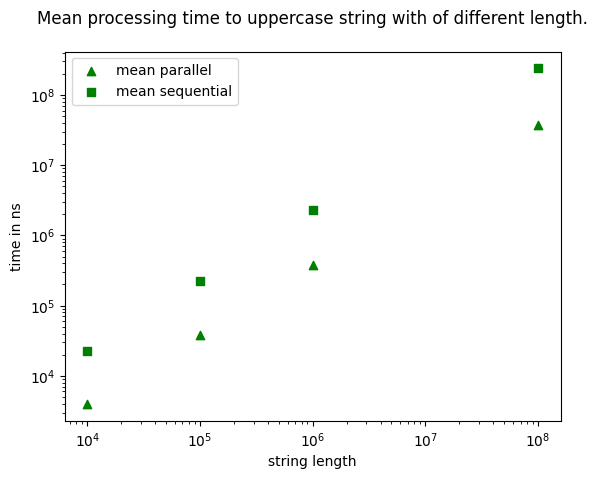
\includegraphics[width=0.7\textwidth]{images/complex_upper.png}
		\caption{Durchschnittliche Durchführungszeit von toUppercase() in Abhängigkeit von der Stringlänge.}
		\label{fig:mean_upper}
	\end{center}
\end{figure}

\begin{figure}[h]
	\begin{center}
		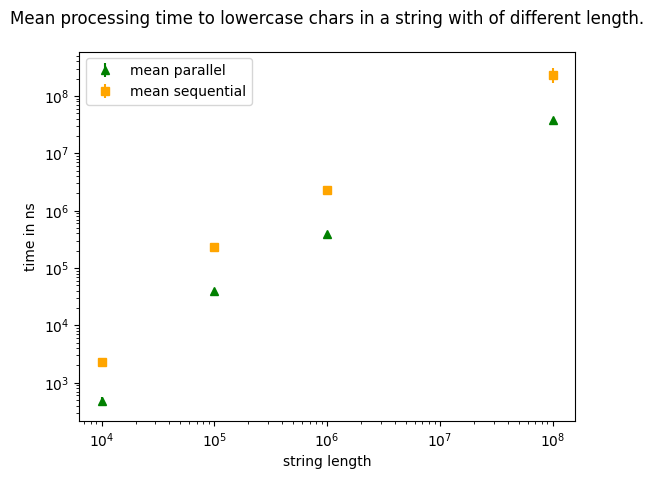
\includegraphics[width=0.7\textwidth]{images/complex_lower.png}
		\caption{Durchschnittliche Durchführungszeit von toLowercase() in Abhängigkeit von der Stringlänge.}
		\label{fig:mean_upper}
	\end{center}
\end{figure}

\begin{figure}[h]
	\begin{center}
		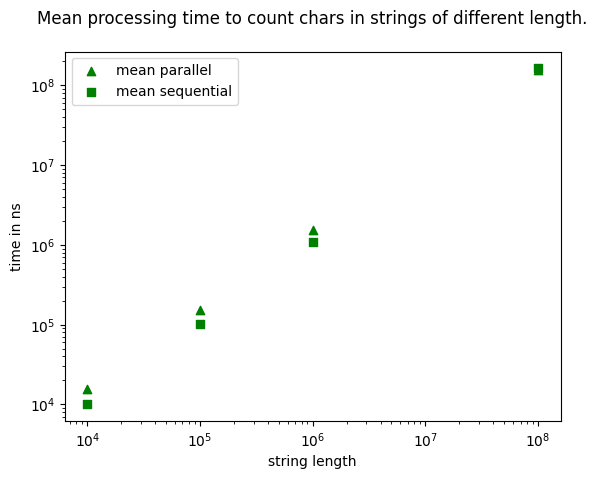
\includegraphics[width=0.7\textwidth]{images/complex_count.png}
		\caption{Durchschnittliche Durchführungszeit von countChar() in Abhängigkeit von der Stringlänge.}
		\label{fig:mean_upper}
	\end{center}
\end{figure}


\subsection{Ausführungszeiten}
\subsubsection{toUppercase}
In der Tabelle \ref{Tab:uppertab} sind die Zeitmessungen für die toUppercase() Funktionen zusammengefasst.
Es ist deutlich zu sehen, dass die se­quen­ti­elle Ausführung in für jede Stringlänge mehr Zeit benötigt als die Umsetzung mit SIMD.
\newline
\begin{tabular}{|c|r|l|r|l|}
	\hline
	\multicolumn{1}{|c|}{String Länge} & \multicolumn{2}{c|}{parallel in ns} & \multicolumn{2}{c|}{se­quen­tiell­ in ns} \\
	\cline{2-5}
	& Mittelwert & Standardabweichung  & Mittelwert & Standardabweichung \\
	\hline
	%\input{tabulars/lower_tab.txt} does some weird stuff and I was unable to figure out why
	10000 & 13812.89 & 2438.83 & 229699.60 & 75923.16 \\
	100000 & 74628.35 & 37815.71 & 791077.37 & 701784.15 \\
	1000000 & 781054.95 & 301556.31 & 7308699.36 & 3514745.39 \\
	100000000 & 56888725.52 & 5992509.42 & 458731319.02 & 61956346.45 \\
	\hline
\end{tabular}
\label{Tab:uppertab}


\subsubsection{toLowercase}
In der Tabelle \ref{Tab:lowertab} sind die Zeitmessungen für die toLowercase() Funktionen zusammengefasst.
Es ist deutlich zu sehen, dass die sequentielle Ausführung in für jede Stringlänge mehr Zeit benötigt als die Umsetzung mit SIMD.
\newline
\begin{tabular}{|c|r|l|r|l|}
	\hline
	\multicolumn{1}{|c|}{String Länge} & \multicolumn{2}{c|}{parallel in ns} & \multicolumn{2}{c|}{sequentiell in ns} \\
	\cline{2-5}
	& Mittelwert & Standardabweichung  & Mittelwert & Standardabweichung \\
	\hline
	%\input{tabulars/upper_tab.txt} does some weird stuff and I was unable to figure out why
	10000 & 13718.13 & 2732.00 & 311293.96 & 435716.85 \\
	100000 & 70663.97 & 33116.91 & 868215.45 & 790953.91 \\
	1000000 & 776718.16 & 328559.81 & 8446686.96 & 4419921.43 \\
	100000000 & 73948537.61 & 9256554.24 & 521830060.76 & 58353286.64 \\
	\hline
\end{tabular}
\label{Tab:lowertab}

\subsubsection{countChar}
In der Tabelle \ref{Tab:counttab} sind die Zeitmessungen für die countChar() Funktionen zusammengefasst.
Es ist zu sehen, dass die sequentielle Ausführung in für jede Stringlänge mehr Zeit benötigt als die Umsetzung mit SIMD. Hier ist der Unterschied allerdings nicht so deutlich wie bei den vorherigen Funktionen. Hier würde es sich lohnen nach einer effizienteren Lösung zu suchen als dem aktuellen Ansatz.
\newline
\begin{tabular}{|c|r|l|r|l|}
	\hline
	\multicolumn{1}{|c|}{String Länge} & \multicolumn{2}{c|}{parallel in ns} & \multicolumn{2}{c|}{sequentiell in ns} \\
	\cline{2-5}
	& Mittelwert & Standardabweichung  & Mittelwert & Standardabweichung \\
	\hline
	%\input{tabulars/count_tab.txt} does some weird stuff and I was unable to figure out why
	10000 & 46062.37 & 5738.73 & 53350.61 & 6362.82 \\
	100000 & 269818.84 & 106161.31 & 322522.16 & 122342.74 \\
	1000000 & 2617943.71 & 559510.81 & 3132603.61 & 554707.70 \\
	100000000 & 206280004.77 & 15598865.64 & 244304383.10 & 12724125.35 \\
	\hline
\end{tabular}
\label{Tab:counttab}

\newpage
\subsection{Vergleich}
In den folgenden Abbildungen sind 100 Laufzeiten für das Verarbeiten eines Strings aufgezeigt. Dabei sind pro Funktion 4 Abbildungen für je 10.000, 100.000, 1.000.000 und 100.000.000 Zeichen in den Strings. Die Diagramme veranschaulichen den Vergleich zwischen dem sequentiellen und parallelen Ansatz unter Verwendung von SIMD.
\subsubsection{toUppercase}
\begin{figure}[h]
	\begin{center}
		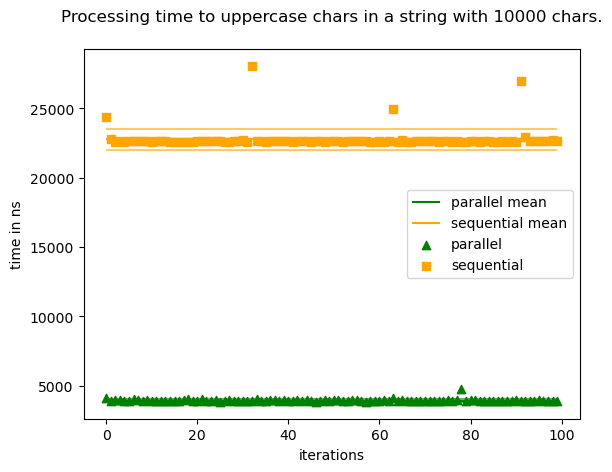
\includegraphics[width=0.65\textwidth]{images/comp_upper_10000.png}
		\caption{Durchführungszeiten von toUppercase für einen String mit 10.000 Zeichen.}
	\end{center}
\end{figure}
\begin{figure}[h]
\begin{center}
	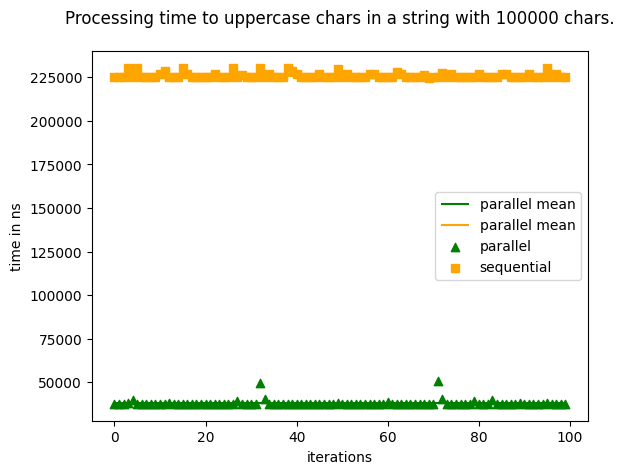
\includegraphics[width=0.65\textwidth]{images/comp_upper_100000.png}
	\caption{Durchführungszeiten von toUppercase für einen String mit 100.000 Zeichen.}
\end{center}
\end{figure}
\begin{figure}[h]
\begin{center}
	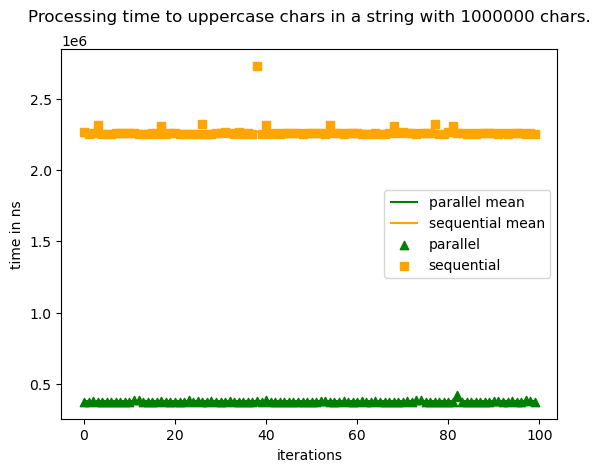
\includegraphics[width=0.65\textwidth]{images/comp_upper_1000000.png}
	\caption{Durchführungszeiten von toUppercase für einen String mit 1.000.000 Zeichen.}
\end{center}
\end{figure}
\begin{figure}[h]
\begin{center}
	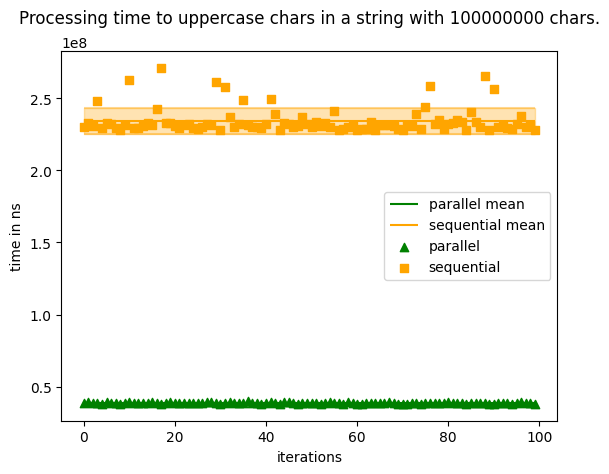
\includegraphics[width=0.65\textwidth]{images/comp_upper_100000000.png}
	\caption{Durchführungszeiten von toUppercase für einen String mit 100.000.000 Zeichen.}
\end{center}
\end{figure}

\clearpage
\subsubsection{toLowercase}
\begin{figure}[h]
	\begin{center}
		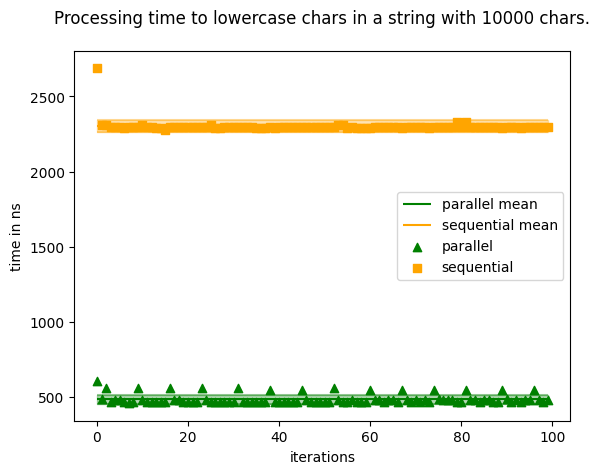
\includegraphics[width=0.65\textwidth]{images/comp_lower_10000.png}
	\end{center}
\end{figure}
\begin{figure}[h]
	\begin{center}
		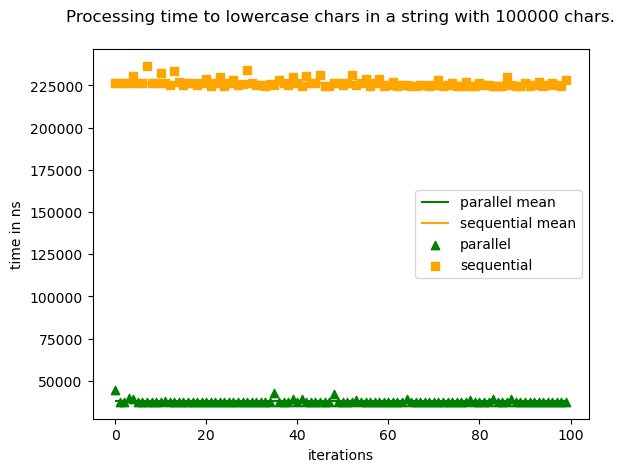
\includegraphics[width=0.65\textwidth]{images/comp_lower_100000.png}
	\end{center}
\end{figure}
\begin{figure}[h]
	\begin{center}
		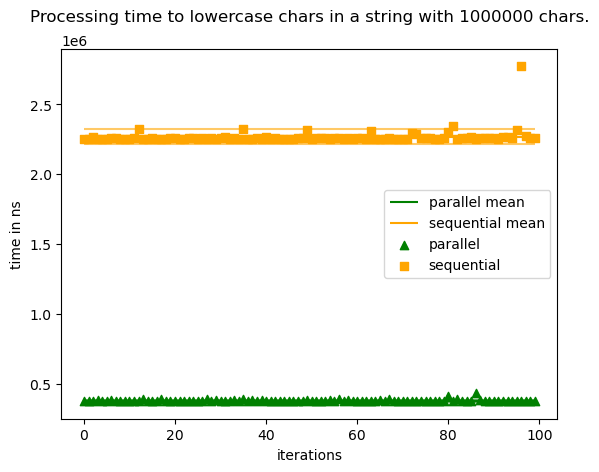
\includegraphics[width=0.65\textwidth]{images/comp_lower_1000000.png}
	\end{center}
\end{figure}
\begin{figure}[h]
	\begin{center}
		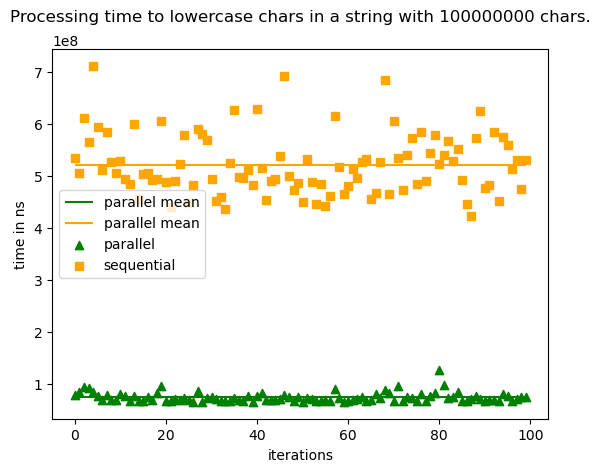
\includegraphics[width=0.65\textwidth]{images/comp_lower_100000000.png}
	\end{center}
\end{figure}

\clearpage
\subsubsection{countChar}
\begin{figure}[h]
	\begin{center}
		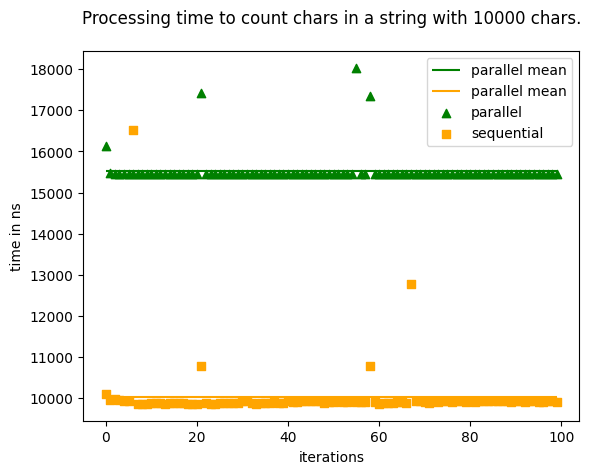
\includegraphics[width=0.65\textwidth]{images/comp_count_10000.png}
	\end{center}
\end{figure}
\begin{figure}[h]
	\begin{center}
		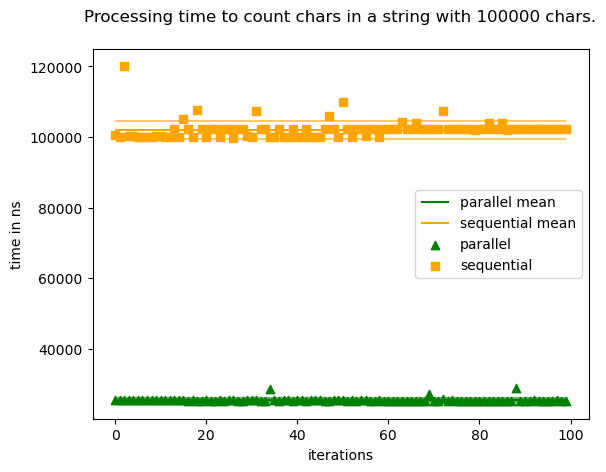
\includegraphics[width=0.65\textwidth]{images/comp_count_100000.png}
	\end{center}
\end{figure}
\begin{figure}[h]
	\begin{center}
		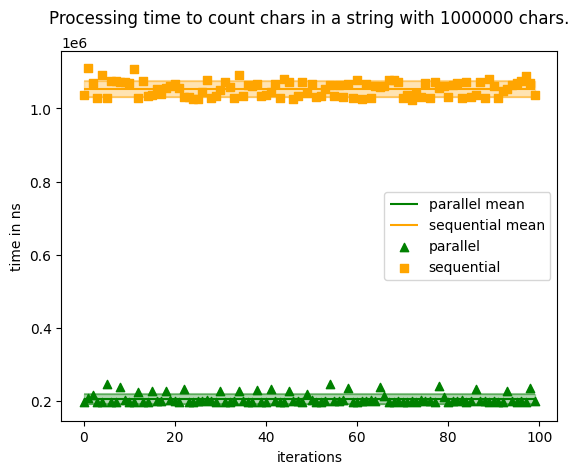
\includegraphics[width=0.65\textwidth]{images/comp_count_1000000.png}
	\end{center}
\end{figure}
\begin{figure}[h]
	\begin{center}
		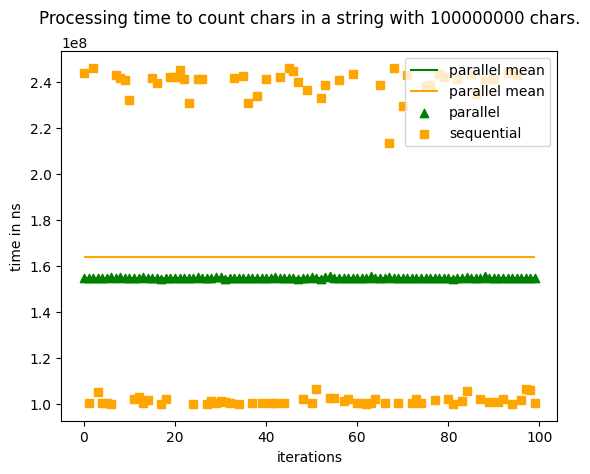
\includegraphics[width=0.65\textwidth]{images/comp_count_100000000.png}
	\end{center}
\end{figure}

\end{document}